\documentclass[11pt,a4paper]{article}

\usepackage{epsfig}
\usepackage{multicol}

\usepackage[utf8]{inputenc}
\usepackage[brazil]{babel}
\usepackage{fancyheadings}
\usepackage{amsmath}
\usepackage{calrsfs}
\usepackage{enumerate}
\DeclareGraphicsExtensions{.png,.pdf}
\usepackage{amsmath, amsfonts, amssymb}
\usepackage{esint}
\usepackage{graphicx}
\usepackage{multicol}
\usepackage{tasks}
\usepackage[utf8]{inputenc}
\usepackage{mathrsfs} % Transformada de Laplace
\usepackage{indentfirst}

% As margens
\setlength{\textheight}{24.0cm}
\setlength{\textwidth}{17.5cm}
\setlength{\oddsidemargin}{2.0cm} % Margens reais desejadas
\setlength{\evensidemargin}{2.0cm} % 2+17.5+1.5=21cm (largura A4)
\setlength{\topmargin}{1.5cm} % 1.5+1.6+1.0+24.0+1.6=29.7cm
\setlength{\headheight}{1.6cm} % (altura A4)
\setlength{\headsep}{1.0cm}
\setlength{\columnsep}{1.5cm} % Coluna = 8cm ((17.5-1.5)/2)
\addtolength{\oddsidemargin}{-1in}
\addtolength{\evensidemargin}{-1in}
\addtolength{\topmargin}{-1in}
\setlength{\footskip}{0.0cm}


% Novos comandos
\newcommand{\limite}{\displaystyle\lim}
\newcommand{\integral}{\displaystyle\int}
\newcommand{\somatorio}{\displaystyle\sum}
\newcommand{\mat}[1]{\mbox{\boldmath{$#1$}}} 

\pagestyle{fancy}


\usepackage{lipsum}

\lhead{

\includegraphics[width=1cm]{brasao.png}
}

\rhead{ 
\sc\textbf{U}niversidade \textbf{F}ederal do \textbf{C}eará\\
Campus Quixadá\\ Monitoria de Cálculo II e III}

\cfoot{}

\begin{document}

	\begin{center}
		\Large Lista 4 - Cálculo III
	\end{center}
	

	\begin{enumerate}
	
	\item Uma carga está distribuída na região triangular $D$ da figura de modo que a densidade de carga em $(x,y)$ é $\sigma (x,y) = xy$, medida em coulombs por metro quadrado $(C/m^2)$. Determine a carga total.

\begin{figure}[h]	
\centering % para centralizarmos a figura	
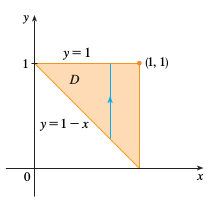
\includegraphics[width=4cm]{Selection_011.png} % leia abaixo
\end{figure}

\item Determine a massa e o centro de massa de uma lâmina triangular com vértices $(0,0),(1,0) \textrm{ e}\ (0,2)$, se a função de densidade for $\rho (x,y) = 1 + 3x + y$.

\item Calcule o centro de massa

\begin{enumerate}
\item $\delta (x,y) = y$ e $B$ o quadrado $0 \leq x \leq 1$, $0 \leq y \leq 1$.
\item $B = \{(x,y) \in \mathbb{R}^2 \,|\, x^2 + 4y^2 \leq 1\ \textrm{,}\ y \geq 0\}$ e a densidade é proporcional à distância do ponto ao eixo $x$.
\item $B$ é o triângulo de vértices $(0,0),(1,0) \textrm{ e}\ (1,1)$ e a densidade é proporcional à distância do ponto à origem.
\item $B$ é o conjunto de todos $(x,y)$ tais que $x^3 \leq y \leq x$ e a densidade é constante e igual a 1.
\item $B$ é o conjunto de todos $(x,y)$ tais que $1 \leq x^2 + y^2 \leq 4$, $y \geq 0$, e a densidade é proporcional à distância do ponto à origem.
\end{enumerate}

\item Calcule

\begin{enumerate}
\item $\displaystyle\iiint_B xyz \,dx\,dy\,dz$ onde $B$ é o paralelepípedo $0 \leq x \leq 2$, $0 \leq y \leq 1$ e $1 \leq z \leq 2$.
\item $\displaystyle\iiint_B x \,dx\,dy\,dz$ onde $B$ é o conjunto $0 \leq x \leq 1$, $0 \leq y \leq 1$ e $x + y \leq z \leq x + y + 1$.
\item $\displaystyle\iiint_B \sqrt{1 - z^2} \,dx\,dy\,dz$ onde $B$ é o conjunto $0 \leq x \leq 1$, $0 \leq z \leq 1$ e $0 \leq z \leq z$.
\item $\displaystyle\iiint_B \sqrt{1 - z^2} \,dx\,dy\,dz$ onde $B$ é o cubo $0 \leq x \leq 1$, $0 \leq y \leq 1$ e $0 \leq z \leq 1$.
\item $\displaystyle\iiint_B \,dx\,dy\,dz$ onde $B$ é o conjunto $x^2 + y^2 \leq z \leq 2x$.
\item $\displaystyle\iiint_B (x^2 + z^2) \,dx\,dy\,dz$ onde $B$ é o cilindro $x^2 + y^2 \leq 1$, $0 \leq z \leq 1$.
\item $\displaystyle\iiint_B \,dx\,dy\,dz$ onde $B$ é o conjunto $x^2 + y^2 \leq z \leq 2x + 2y - 1$.
\item $\displaystyle\iiint_B (x^2 + z^2)\,dx\,dy\,dz$ onde $B$ é o cilindro $x^2 + y^2 \leq 1$, $0 \leq z \leq 1$.
\item $\displaystyle\iiint_B x \,dx\,dy\,dz$ onde $B$ é o conjunto $x^2 - y^2 \leq z \leq 1 - 2y^2$.
\item $\displaystyle\iiint_B x \,dx\,dy\,dz$ onde $B$ é o conjunto $x^2 \leq y   \leq x$, $0 \leq z \leq x + y$.
\item $\displaystyle\iiint_B 2z \,dx\,dy\,dz$ onde $B$ é o conjunto $4x^2 + 9y^2 + z^2 \leq 4$, $z \geq 0$.

\end{enumerate}

\item Calcule a integral abaixo
$$\displaystyle\iiint_B (y - x) \,dx\,dy\,dz$$

onde $B$ é o conjunto $4 \leq x + y \leq 8$, $\dfrac{1}{x} \leq y \leq \dfrac{2}{x}$, $y > x$ e $0 \leq z \leq \dfrac{\sqrt[3]{xy}}{\sqrt{x + y}}$.

\item Calcule o volume do conjunto dado. 

\begin{enumerate}

\item $0 \leq x \leq 1$, $0 \leq y \leq 1$ e $0 \leq z \leq 5 - x^2 - 3y^2$.
\item $0 \leq x \leq 1$, $0 \leq y \leq x^2$ e $0 \leq z \leq x + y^2$.
\item $x^2 + y^2 \leq z \leq 4$.
\item $x^2 + y^2 \leq z \leq 1$.
\item $x^2 + y^2 \leq 4$ e $x^2 + y^2 + z^2 \leq 9$.
\item $\dfrac{x^2}{a^2} + \dfrac{y^2}{b^2} + \dfrac{z^2}{c^2} \leq 1$ onde $(a > 0 \textrm{,}\ b > 0 \textrm{ e}\ c > 0)$.
\item $x^2 + y^2 \leq z \leq 4x + 2y$.
\item $(x-a)^2 + y^2 \leq a^2$, $x^2 + y^2 + z^2 \leq 4a^2$, $z \geq 0$ com $a > 0$.
\item $x^2 + y^2 + z^2 \leq a^2$ e $\dfrac{a}{2}$ com $(a > 0)$.
\item $x^2 + 2y^2 \leq z \leq 2a^2 - x^2$ com $(a > 0)$.
\item $4x^2 + 9y^2 + z^2 \leq 4$ e $4x^2 + 9y^2 \leq 1$.

\end{enumerate}

\item Calcule a massa do cubo $0 \leq x \leq 1$, $0 \leq y \leq 1$ e $0 \leq z \leq 1$, cuja densidade no ponto $(x,y,z)$ é a soma das coordenadas.

\item Calcule a massa do sólido $x + y + z \leq 1$, $x \geq 0$, $y \geq 0$ e $z \geq 0$, sendo a densidade dada por $\delta (x,y,z) = x + y$.

\item Calcule a massa do cilindro $x^2 + y^2 \leq 4$ e $0 \leq z \leq 2$, sabendo que a densidade no ponto $(x,y,z)$ é o dobro da distância do ponto ao plano $z = 0$.

\item Calcule a massa do cone $\sqrt{x^2 + y^2} \leq z \leq 1$, sendo a densidade no ponto $(x, y, z)$ proporcional ao quadrado da distância do ponto ao eixo $z$.

\item Calcule

\begin{enumerate}

\item $\displaystyle\iiint_B x \,dx\,dy\,dz$ onde $B$ é o conjunto $x \geq 0$, $x^2 + y^2 + z^2 \leq 4$.
\item $\displaystyle\iiint_B z \,dx\,dy\,dz$ onde $B$ é o conjunto $1 \leq x^2 + y^2 + z^2 \leq 4$, $z \geq 0$.
\item $\displaystyle\iiint_B x \,dx\,dy\,dz$ onde $B$ é o conjunto $\dfrac{x^2}{4} + \dfrac{y^2}{9} + z^2 \leq 1$, $x \geq 0$.
\item $\displaystyle\iiint_B z \,dx\,dy\,dz$ onde $B$ é o conjunto $z \geq \sqrt{x^2 + y^2}$, $x^2 + y^2 + z^2 \leq 1$.
\item $\displaystyle\iiint_B \sqrt{x^2 + y^2 + z^2} \,dx\,dy\,dz$ onde $B$ é a intersecção da semi-esfera $x^2 + y^2 + z^2 \leq 4$, $z \geq 0$, com o cilindro $x^2 + y^2 \leq 1$.

\end{enumerate}

\item Calcule o volume do elipsóide $\dfrac{x^2}{a^2} + \dfrac{y^2}{b^2} + \dfrac{z^2}{c^2} \leq 1$.

\item Calcule o volume do conjunto $z \geq \sqrt{x^2 + y^2}$ e $x^2 + y^2 + z^2 \leq 2az$ com $(a > 0)$.

\item Mostre que
$$\integral_{-\infty}^{+\infty} \integral_{-\infty}^{+\infty} \integral_{-\infty}^{+\infty} \sqrt{x^2 + y^2 + z^2} \ e^{-(x^2 + y^2 + z^2)} \,dx\,dy\,dz = 2 \pi$$

(A integral imprópria tripla é definida como o limite da integral tripla sobre uma esfera sólida quando o raio da esfera aumenta indefinidamente.)

\item Demonstre a integral de densidade probabilidade abaixo
$$\integral_{-\infty}^{+\infty} e^{-x^2}\,dx = \sqrt{\pi}$$ 
\end{enumerate}
		
	
\end{document}